\chapter{Pin-Injection Automation für Diehl Aviation}
\label{ch:pia}

Das zu programmierende Projekt \ac{pia} wird für den Kunden Diehl Aviation\footnote{\url{https://www.diehl.com/aviation/de/}} entwickelt, welches als semi-automatisiertes Pin Injection Testing Programm fungieren soll.

Der Kunde Diehl muss die von ihnen entwickelten Geräte auf viele bestimmte Eigenschaften und Ereignisse \ac{bzw} auch auf Gefahren testen, welche während eines Fluges auftreten können. Einer dieser Tests ist der sogenannte Pin-Injection Test.
Bei diesem Test werden die Pins eines Fluggerätes auf Störungen und auch Beschädigungen im Rahmen der Umweltqualitätsprüfung nach \cite{DO-160} getestet. Jeder Pin besitzt ein Interface zum steuern von verschiedenen im Gerät verbauten Schaltern. Da jedes Interface andere Eigenschaften besitzt, hat dementsprechend jedes dieser Interfaces unterschiedliche Anforderungen (engl: "Requirements") die getestet werden müssen.
Demzufolge ist das Testen der Pins \ac{bzw} der Geräte sehr zeitaufwändig und kann im Durchschnitt bis zu zwei Wochen dauern, je nachdem wie viele Pins das zu testende Gerät besitzt.

\ac{pia} soll die Tests, welche normalerweise von einem Mitarbeiter von Hand abgearbeitet werden, einlesen und nur durch eine vom Mitarbeiter angefertigte Konfigurationsdatei automatisieren und verarbeiten.


\section{Projekteinarbeitung}
\label{sec:prj-einarbeitung}

Da das Projekt erst kurz vor meinem ersten Arbeitstag angenommen und mit Diehl beschlossen wurde, stand bis auf die Aufgabenanforderung der Software noch nichts fest. Dementsprechend konnte ich später in vielen Bereichen wie \ac{zb} die Programmiersprache oder auch die Programmstruktur frei wählen und auch viele meiner Ideen mit ins Programm einfließen lassen. Meine erste Aufgabe war es erst einmal das Verständnis für den eigentlichen Test zu bekommen, welcher das Programm automatisieren soll, denn zu diesem Zeitpunkt war der vom Programm abzulaufende Testzyklus noch nicht vollständig festgelegt. 


\subsection{Aufgabe der zu programmierenden Software}
\label{subsec:aufgabe-software}

Die Aufgabe der zu entwickelten Software besteht darin, dass eine vom Mitarbeiter erstellte Testkonfigurationsdatei, welche normalerweise von Hand abgearbeitet wird, eingelesen und verarbeitet wird. Am Ende soll eine sogenannte Result Ouput Log File die Ausgaben der Programmauswertung abspeichern und angeben ob ein Test gescheitert ist oder alles normal verlief.
Bei der Verarbeitung eines Test Schritts wird ein Roboter angesteuert der maximal zwei sogenannte Bananenstecker auf ein Board steckt, welches mit den Pins des zu testenden Gerätes angeschlossen ist. Danach kann ein optionales \ac{micbac} Kommando an das am Pin anliegende Interface geschickt werden, welches \ac{zb} einen internen Schalter umlegt. Danach wird ein Puls mehrmals auf den Pin gefeuert. Dieser Puls hat eine vorgegebene Wellenform (engl: "Waveform"), welche von einem angeschlossen Puls Generator generiert wird. Der Puls Generator ist zugleich auch für die Anzahl der zu feuernden Pulse zuständig. Nach dem letzten abgefeuerten Puls wird ein Bild vom Oszilloskop abgespeichert und mit einem vorher aufgenommenen Referenzbild verglichen, um zu schauen ob der Pin \ac{bzw} sogar das komplette Gerät beschädigt wurde oder ob alles in normal verlaufenden Bereich liegt. 


\subsection{Entwicklung der Programmstruktur}
\label{subsec:entw-prgstr}

Während meiner Praxisphase war die Entwicklung und im späteren Verlauf auch die Weiterentwicklung der Programmstruktur ein großer Bestandteil meiner Arbeit. Da die Entwicklung zum Teil etappenmäßig voran ging, mussten Teile der Programmstruktur relativ schnell und ohne wirklich großen Aufwand modifizierbar, erweiterbar und zu einem gewissen Teil auch austauschbar sein. Abbildung \ref{fig:prg_architecture} zeigt die entwickelte abstrakte Programmstruktur, welche im Programm auch umgesetzt und benutzt wurde. Dort sieht man auch, dass das Programm mehrere Interfaces für Oszilloskope und Puls-Generatoren ansteuert. Diese Anforderung wurde am Ende so implementiert, dass sofern irgendeine neue Hardware Komponente eingebettet werden soll, nur kleine Teile wie \ac{zb} die Auswahlmöglichkeit in der \ac{gui} erweitert werden muss. Die eigentliche Programmstruktur wird dadurch nicht verändert, was die Flexibilität erhöht und es so möglich ist das Programm nur durch hinzufügen einer neuen Datei, unter der Einhaltung von einer bestimmten  Namensvergebung, zu erweitern. Erkennbar ist auch, dass die Aufgaben in unterschiedliche Interfaces unterteilt wurden, was die Programmübersicht erhöht und  interne Abhängigkeiten verringert. Dadurch sind \ac{zb} teile der \ac{gui} des öfteren ohne großen aufwand schnell austauschbar gewesen, was mir im Verlaufe des Praktikums öfters mal sehr viel Zeit eingespart hat.

\begin{figure}[H]
	\centering
	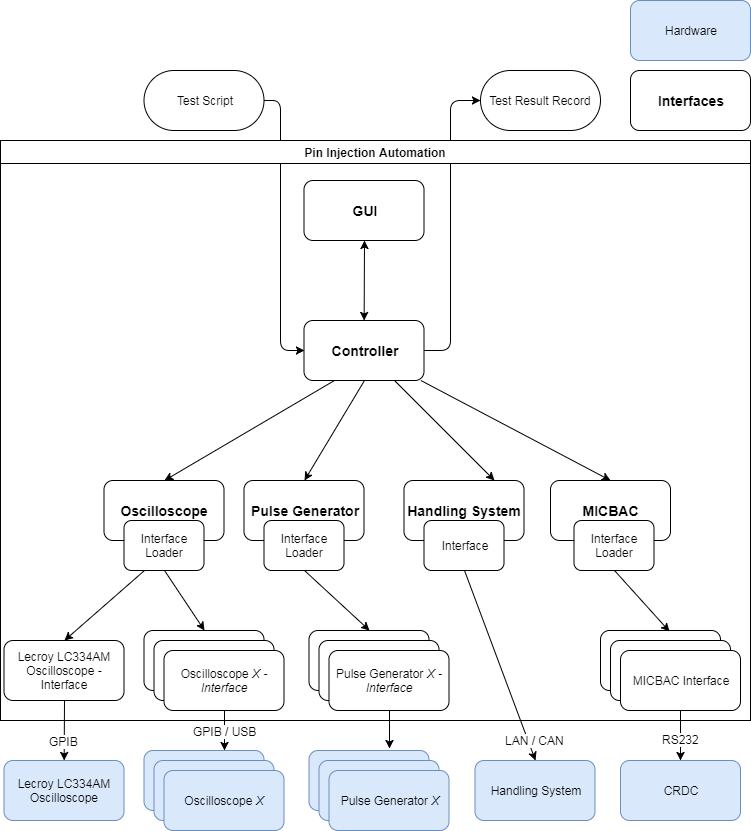
\includegraphics[width=0.75\textwidth, height=0.75\textwidth]{graphics/program_architecture.png}
	\caption{Programm Architektur}
	\label{fig:prg_architecture}
\end{figure}
	
\subsection{Python 3 als Programmiersprache}
\label{subsec:py3_as_lang}

\citetitle{python35}
